% ===== Styles pgfplots pour les graphiques du chapitre =====
\pgfplotsset{
	repere/.style={
		axis lines=middle,
		axis line style={-stealth},
		grid=both,
		grid style={gray!25},
		minor tick num=0,
		tick label style={font=\scriptsize, fill=white, inner sep=1pt},
		xlabel={}, ylabel={},
		samples=150,
		clip=true,
	},
	courbe/.style={very thick, smooth},
}

\chapter{Fonctions polynôme de dégré 2}
\thispagestyle{fancy}

\vspace*{-0.5cm}
\section{Définition}

	\vspace*{-0.2cm}
    \begin{bdefi}
        On appelle \grasInDef{fonction polynôme de degré 2} toute fonction f définie sur \R par une expression de la forme :\\
				\grasInDef{$\bm{f(x)=ax^2+bx+c}$}
        où les coefficients $a$, $b$ et $c$ sont des réels donnés avec $a\neq0$.
    \end{bdefi}
    
    \begin{brmq}
        Une fonction polynôme de degré 2 s'appelle également fonction trinôme du second degré ou par abus de langage \guillemets{trinôme}.
    \end{brmq}
    
    \begin{bexemples}
    	
    	\setlength{\extrarowheight}{2pt}
        \begin{tabular}[t]{|Xc|Xc|Xc|Xc|Xc|Xc|}
        	\hline \multirow[b]{2}{*}{$f(x)=\ldots$} & \multicolumn{2}{|c|}{$f$ fonction polynôme de degré 2 ?} & $a=$ ? & $b=?$ & $c=?$ \\
        	\hline & oui & non & & & \\
        	\hline $2 x^2-5 x+3$ & X & &2 &$-5$ & 3\\
        	\hline $x^2$ & X & & 1& 0& 0\\
        	\hline $3 x^3+6 x-1$ & & X& & & \\
        	\hline $2 x+3-x^2$ & X & & $-1$& 2& 3\\
        	\hline $(2 x+1)(2-3 x)$ & X & & $-6$ & 1& 2\\
        	\hline $3 x^2+1$ & X & & 3 & 0 & 1 \\
        	\hline $3 x+7$ & & X & & & \\
        	\hline
        \end{tabular}
    \end{bexemples}

	\section{Représentation graphique}
	
	\subsection{La parabole}
	
	\begin{bdefi}
		La courbe représentative d'une fonction polynôme du second degré est appelée \grasInDef{parabole}.
	\end{bdefi}
	
%	\includegraphics[scale=0.2]{6565556a-62f8-4538-9b1a-28dfdf48b958-1_700_986_2017_888}
	
	\begin{bprops}
		Soit $f$ une fonction polynôme du second degré, telle que $f(x)=a x^{2}+b x+c$.
		
		\begin{itemProp}
			\item Si $a$ est positif, $f$ est d'abord décroissante, puis croissante.
			\item Si $a$ est négatif, $f$ est d'abord croissante, puis décroissante.
		\end{itemProp}
	\end{bprops}	
	
	\begin{minipage}[c]{0.48\linewidth}
		$$
		a>0
		$$
		
		\begin{center}
			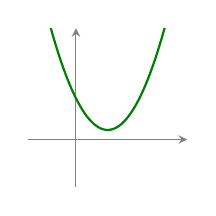
\begin{tikzpicture}
				\begin{axis}[axis lines=middle, axis line style={gray}, ticks=none,
					width=3.6cm, height=3.6cm, xmin=-1.5, xmax=3.5, ymin=-1.5, ymax=3.5]
					\addplot[green!50!black, thick, smooth, domain=-1.5:3.5, samples=80] {(x-1)^2+0.3};
				\end{axis}
			\end{tikzpicture}
		\end{center}
		
		Les branches de la parabole sont tirées vers le haut.
	\end{minipage} \hfill
	\begin{minipage}[c]{0.48\linewidth}
		$$
		a<0
		$$
		
		\begin{center}
			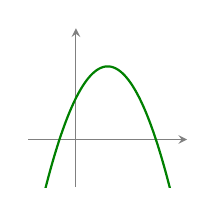
\begin{tikzpicture}
				\begin{axis}[axis lines=middle, axis line style={gray}, ticks=none,
					width=3.6cm, height=3.6cm, xmin=-1.5, xmax=3.5, ymin=-1.5, ymax=3.5]
					\addplot[green!50!black, thick, smooth, domain=-1.5:3.5, samples=80] {-(x-1)^2+2.3};
				\end{axis}
			\end{tikzpicture}
		\end{center}
		
		Les branches de la parabole sont tirées vers le bas.
	\end{minipage}
	
	\begin{center}
		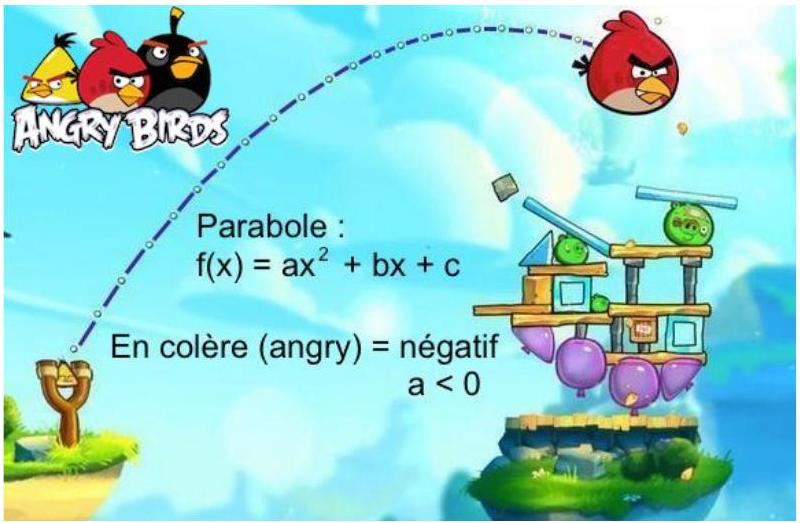
\includegraphics[scale=0.25]{angry_birds}
	\end{center}
	
	
	
	\subsection{Axe de symétrie et sommet de la courbe}
	
	\begin{minipage}[c]{0.48\linewidth}
		La courbe d'une fonction polynôme du second degré possède un axe de symétrie.
		
		Le sommet de la courbe se trouve à l'intersection de l'axe de symétrie avec la courbe.
	\end{minipage} \hfill
	\begin{minipage}[c]{0.48\linewidth}
		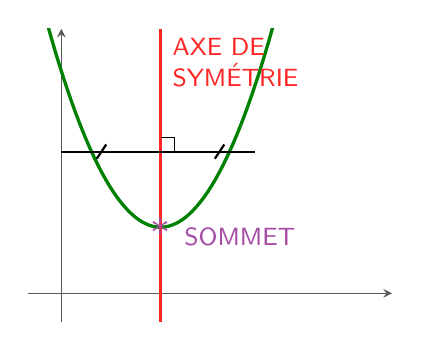
\begin{tikzpicture}[scale=0.6]
			% repère
			\draw[-stealth, gray!70!black] (-1.2,-0.4) -- (6.5,-0.4);
			\draw[-stealth, gray!70!black] (-0.5,-1) -- (-0.5,5.2);
			% parabole
			\begin{scope}
				\clip (-1.2,-1) rectangle (6.5,5.2);
				\draw[green!50!black, very thick, domain=-1:4.2, samples=100, smooth] plot (\x,{0.75*(\x-1.6)*(\x-1.6)+1});
			\end{scope}
			% axe de symétrie
			\draw[red!85!white, thick] (1.6,-1) -- (1.6,5.2);
			\node[red!85!white, font=\sffamily\small, align=left, anchor=north west] at (1.65,5.2) {AXE DE\\SYMÉTRIE};
			% segment horizontal et codage
			\draw[thick] (-0.5,2.6) -- (3.6,2.6);
			\draw[thick] (0.25,2.45) -- (0.45,2.75);
			\draw[thick] (2.75,2.45) -- (2.95,2.75);
			\draw (1.6,2.9) -- (1.9,2.9) -- (1.9,2.6);
			% sommet
			\node[violet!70!white, font=\Large] at (1.6,1) {$\ast$};
			\node[violet!70!white, font=\sffamily\small, anchor=west] at (1.9,0.8) {SOMMET};
		\end{tikzpicture}
	\end{minipage}
	
	\begin{bmethodet}{Déterminer les éléments caractéristiques d'une parabole}
		\grasInMet{Enoncé:}
		
		\begin{minipage}[c]{0.48\linewidth}
			On a représenté la fonction polynôme du second degré $f$ définie par $f(x)=x^{2}+3 x-2$.
			\begin{enumMet}
				\item Déterminer graphiquement les solutions de l'équation $f(x)=2$.
				\item Tracer l'axe de symétrie de la courbe.
				\item Donner les coordonnées du sommet de la courbe.
			\end{enumMet}
		\end{minipage} \hfill
		\begin{minipage}[c]{0.48\linewidth}
			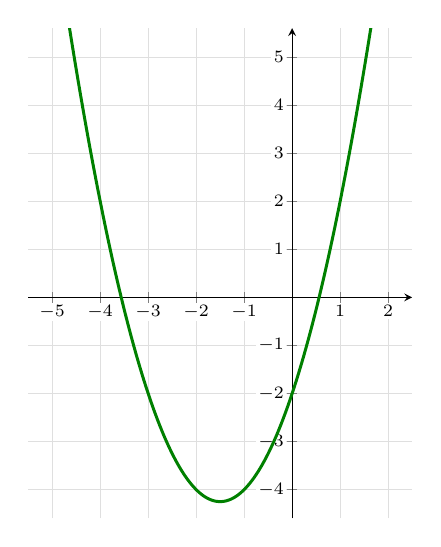
\begin{tikzpicture}[scale=0.9]
				\begin{axis}[repere, width=7cm, height=8.5cm,
					xmin=-5.5, xmax=2.5, ymin=-4.6, ymax=5.6,
					xtick={-5,...,2}, ytick={-4,...,5}]
					\addplot[courbe, green!50!black, domain=-5.5:2.5] {x^2+3*x-2};
				\end{axis}
			\end{tikzpicture}
		\end{minipage}
		
		\grasInMet{Réponse:}
		
		\begin{minipage}[c]{0.48\linewidth}
			\begin{enumMet}
				\item Les solutions de l'équation $f(x)=2$ sont $x=-4$ et $x=1$.
				\item L'axe de symétrie de la courbe est la droite verticale qui coupe l'axe des abscisses en -1,5.\\
				En effet : $(-4+1): 2=-1,5$.
				\item Le sommet est à l'intersection de l'axe de symétrie avec la courbe. Donc son abscisse est -1,5.\\
				Son ordonnée est :
				$$
				f(-1,5)=(-1,5)^{2}+3 \times(-1,5)-2=-4,25 .
				$$
				
				Les coordonnées du sommet sont donc :
				
				$$
				(-1,5 ;-4,25) .
				$$
			\end{enumMet}
		\end{minipage} \hfill
		\begin{minipage}[c]{0.48\linewidth}
			\begin{center}
				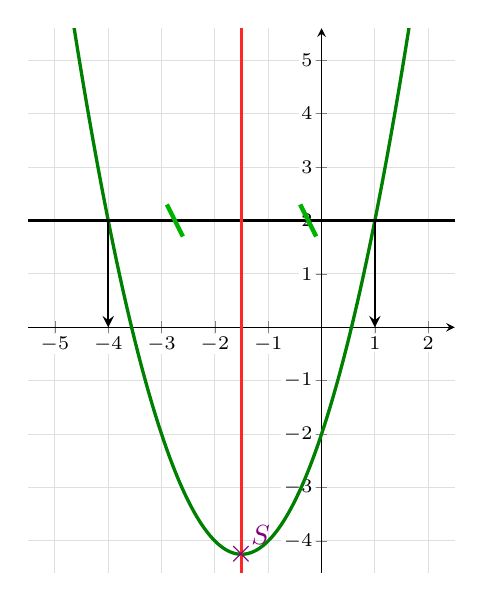
\begin{tikzpicture}
				\begin{axis}[repere, width=7cm, height=8.5cm,
					xmin=-5.5, xmax=2.5, ymin=-4.6, ymax=5.6,
					xtick={-5,...,2}, ytick={-4,...,5}]
					\addplot[courbe, green!50!black, domain=-5.5:2.5] {x^2+3*x-2};
					% droite y = 2
					\addplot[thick, black, domain=-5.5:2.5] {2};
					% solutions
					\draw[-stealth, thick] (axis cs:-4,2) -- (axis cs:-4,0);
					\draw[-stealth, thick] (axis cs:1,2) -- (axis cs:1,0);
					% axe de symétrie
					\draw[red!85!white, thick] (axis cs:-1.5,-4.6) -- (axis cs:-1.5,5.6);
					% codage des longueurs égales
					\draw[green!70!black, ultra thick] (axis cs:-2.9,2.3) -- (axis cs:-2.6,1.7);
					\draw[green!70!black, ultra thick] (axis cs:-0.4,2.3) -- (axis cs:-0.1,1.7);
					% sommet
					\node[violet, font=\large] at (axis cs:-1.5,-4.25) {$\times$};
					\node[violet, anchor=south west] at (axis cs:-1.5,-4.25) {$S$};
				\end{axis}
			\end{tikzpicture}
			\end{center}
		\end{minipage}
		
	\end{bmethodet}
	
	\begin{bprop}
		\grasInProp{L'axe de symétrie} d'une courbe représentative d'une fonction polynôme du second degré définie par $f(x)=a x^{2}+c$ est l'axe des ordonnées et son sommet est le point de coordonnées $(0 ; c)$.
	\end{bprop}
	
	\begin{bmethodet}{Associer une fonction du second degré à sa représentation graphique}
		\grasInMet{Enoncé:}
		
		\begin{minipage}[c]{0.42\linewidth}
			Associer chaque fonction à sa représentation graphique :
			
			$$
			\begin{aligned}
				& f(x)=-x^{2}+3 \\
				& g(x)=-3 x^{2} \\
				& h(x)=x^{2}+3 \\
				& p(x)=\frac{x^{2}}{4}+1 \\
				& q(x)=-\frac{x^{2}}{4}+1
			\end{aligned}
			$$
		\end{minipage} \hfill
		\begin{minipage}[c]{0.58\linewidth}
			\begin{center}
				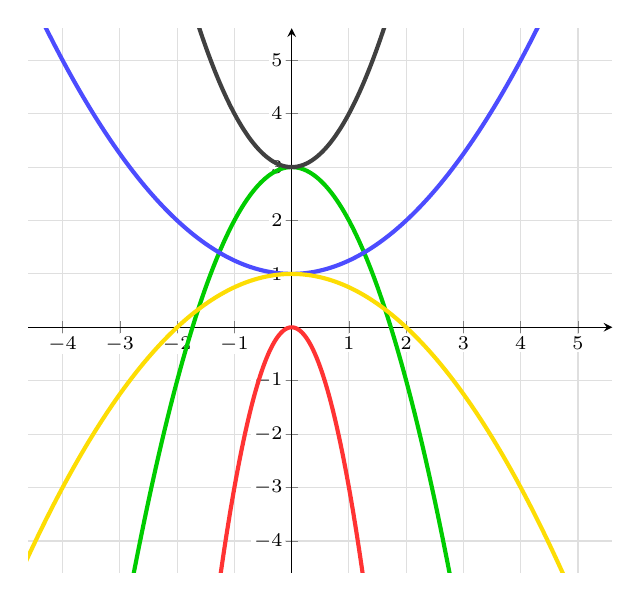
\begin{tikzpicture}
					\begin{axis}[repere, width=9cm, height=8.5cm,
						xmin=-4.6, xmax=5.6, ymin=-4.6, ymax=5.6,
						xtick={-4,...,5}, ytick={-4,...,5}]
						\addplot[courbe, green!80!black, line width=1.5pt, domain=-3:3] {-x^2+3};
						\addplot[courbe, red!80!white, line width=1.5pt, domain=-1.5:1.5] {-3*x^2};
						\addplot[courbe, black!75, line width=1.5pt, domain=-2:2] {x^2+3};
						\addplot[courbe, blue!70!white, line width=1.5pt, domain=-5:5.6] {x^2/4+1};
						\addplot[courbe, yellow!80!orange, line width=1.5pt, domain=-5:5.6] {-x^2/4+1};
					\end{axis}
				\end{tikzpicture}
			\end{center}
		\end{minipage}
		
		\grasInMet{Réponse:}
		
	\begin{itemMet}
		\item La parabole rouge est la seule dont le sommet est l'origine (0 ; 0). Donc $c=\mathbf{0}$ dans l'écriture de la fonction $x \mapsto a x^{2}+c$.\\
		Ainsi, la parabole rouge représente la fonction $g$ définie par $g(x)=-3 x^{2}$.
		\item La parabole verte et la parabole noire ont toutes les deux pour sommet le point de coordonnées ( 0 ; 3).\\
		Donc $c=\mathbf{3}$ dans l'écriture de la fonction $x \mapsto a x^{2}+c$.\\
		Ainsi, il faut choisir parmi les expressions : $f(x)=-x^{2}+3$ et $h(x)=x^{2}+3$.
		\item Les branches de la parabole noire sont tournées vers le haut donc $a>0$ dans l'écriture de la fonction $x \mapsto a x^{2}+c$.\\
		Ainsi, la parabole noire représente la fonction $h$ pour qui $a=1>0$.
		\item Les branches de la parabole verte sont tournées vers le bas donc $a<0$.\\
		Ainsi, la parabole verte représente la fonction $f$ pour qui $a=-1<0$.
		\item La parabole bleue et la parabole jaune ont toutes les deux pour sommet le point de coordonnées ( 0 ; 1).\\
		Donc $c=\mathbf{1}$ dans l'écriture de la fonction $x \mapsto a x^{2}+c$.\\
		Ainsi, il faut choisir parmi les expressions : $p(x)=\frac{x^{2}}{4}+1$ et $q(x)=-\frac{x^{2}}{4}+1$.
		\item Les branches de la parabole bleue sont tournées vers le haut donc $a>0$ dans l'écriture de la fonction $x \mapsto a x^{2}+c$.\\
		Ainsi, la parabole bleue représente la fonction $p$ pour qui $a=\frac{1}{4}>0$.
		\item Les branches de la parabole jaune sont tournées vers le bas donc $a<0$.\\
		Ainsi, la parabole jaune représente la fonction $q$ pour qui $a=-\frac{1}{4}<0$.
	\end{itemMet}
		
	\end{bmethodet}
	
	\subsection{Tableau de variations}
	
	\begin{bprop}
		Soit $f$ une fonction polynôme du second degré définie sur $\mathbb{R}$ par $f(x)=a x^{2}+b x+c$.\\
		\begin{minipage}[c]{0.5\linewidth}
			Si $a>0$
			\ \\
			
			\begin{tikzpicture}
				\tikzset{node style/.append style = {fill=none}}
				\tkzTabInit[lgt = 1.6, espcl = 2.4, deltacl = 0.5]{$x$ / 1 , $f(x)$ / 2}{$-\infty$, $x_S$, $+\infty$}
				\tkzTabVar{+/, -/ $y_S$, +/ }
			\end{tikzpicture}
		\end{minipage}
		\begin{minipage}[c]{0.5\linewidth}
			Si $a<0$
			\ \\
			
			\begin{tikzpicture}
				\tikzset{node style/.append style = {fill=none}}
				\tkzTabInit[lgt = 1.6, espcl = 2.4, deltacl = 0.5]{$x$ / 1 , $f(x)$ / 2}{$-\infty$, $x_S$, $+\infty$}
				\tkzTabVar{-/, +/ $y_S$, -/ }
			\end{tikzpicture}
		\end{minipage}
	\end{bprop}
	
	\begin{bdefi}
		le point de coordonnés $\left(x_S ; y_S\right)$ avec $y_S$ l'extremum de $f$ sur $\mathrm{P}$ est appelé \grasInDef{sommet de la parabole}.
	\end{bdefi}
	
	\begin{bexemple}
		On donne le tableau de variations de la fonction polynôme du second degré $f$.
		\begin{minipage}[c]{0.48\linewidth}
			\begin{tikzpicture}
				\tikzset{node style/.append style = {fill=none}}
				\tkzTabInit[lgt = 1.6, espcl = 2.4, deltacl = 0.5]{$x$ / 1 , $f(x)$ / 2}{$-\infty$, $3$, $+\infty$}
				\tkzTabVar{+/, -/ $-1$, +/ }
			\end{tikzpicture}
			
			Le point de coordonnées (3 ; $-1$) est le sommet S de la courbe.\\
			L'axe de symétrie est la droite verticale qui coupe l'axe des abscisses en 3.\\
		\end{minipage} \hfill
		\begin{minipage}[c]{0.48\linewidth}
			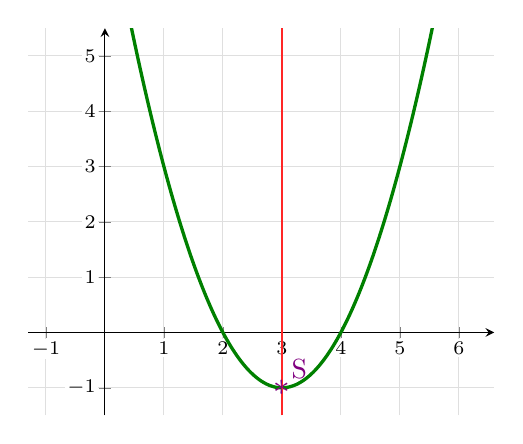
\begin{tikzpicture}
					\begin{axis}[repere, width=7.5cm, height=6.5cm,
						xmin=-1.3, xmax=6.6, ymin=-1.5, ymax=5.5,
						xtick={-1,...,6}, ytick={-1,...,5}]
						\addplot[courbe, green!50!black, domain=-1.3:6.6] {(x-3)^2-1};
						\draw[red!85!white, thick] (axis cs:3,-1.5) -- (axis cs:3,5.5);
						\node[violet, font=\large] at (axis cs:3,-1) {$\ast$};
						\node[violet, anchor=south west] at (axis cs:3,-1) {S};
					\end{axis}
				\end{tikzpicture}
		\end{minipage}
		
	\end{bexemple}
	
	\section{Forme factorisée d'une fonction polynôme de degré 2}
	
	\begin{bexemple}
		La fonction $f$ définie par $f(x)=2(x-3)(x+2)$ est une fonction du second degré.\\
		En effet, elle s'écrit aussi sous la forme $x \mapsto a x^{2}+b x+c$.
		$$
		f(x)=2(x-3)(x+2)=2\left(x^{2}+2 x-3 x-6\right)=2 x^{2}-2 x-12 .
		$$
	\end{bexemple}
	
	\begin{bdefi}
		Une fonction définie sur $\mathbb{R}$ par $f(x)=a\left(x-x_{1}\right)\left(x-x_{2}\right)$ est une fonction polynôme de degré 2 écrite sous sa \grasInDef{forme factorisée}.
	\end{bdefi}
	
	\begin{bprop}
		Soit la fonction $f$ définie sur $\mathbb{R}$ par $f(x)=a\left(x-x_{1}\right)\left(x-x_{2}\right)$.\\
		L'équation $f(x)=0$ possède deux solutions (éventuellement égales) : $x=x_{1}$ et $x=x_{2}$ appelées \grasInProp{les racines} de la fonction polynôme $f$.
	\end{bprop}
	
	\begin{bmethodet}{Associer une fonction du second degré à sa représentation graphique}
		\grasInMet{Enoncé:}
		
		\begin{minipage}[c]{0.42\linewidth}
			Associer chaque fonction à sa représentation graphique :
			
			$$
			\begin{aligned}
				& f(x)=3(x-1)(x+3) \\
				& g(x)=-2(x-1)(x+3) \\
				& h(x)=5(x-1)^{2}
			\end{aligned}
			$$
		\end{minipage} \hfill
		\begin{minipage}[c]{0.58\linewidth}
			\begin{center}
				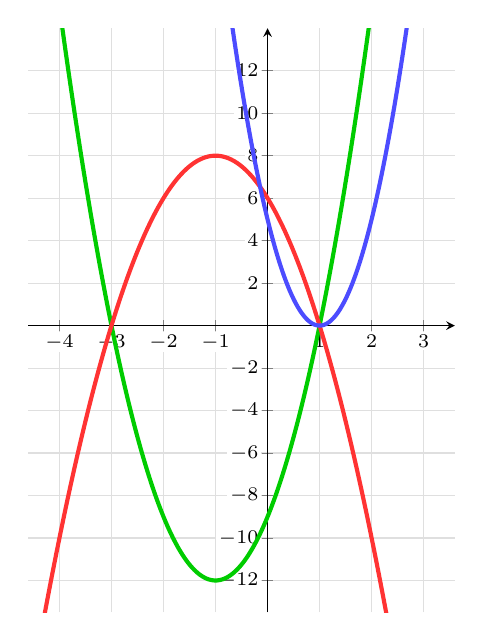
\begin{tikzpicture}
					\begin{axis}[repere, width=7cm, height=9cm,
						xmin=-4.6, xmax=3.6, ymin=-13.5, ymax=14,
						xtick={-4,...,3}, ytick={-12,-10,...,12}]
						\addplot[courbe, green!80!black, line width=1.5pt, domain=-4.6:3.6] {3*(x-1)*(x+3)};
						\addplot[courbe, red!80!white, line width=1.5pt, domain=-4.6:3.6] {-2*(x-1)*(x+3)};
						\addplot[courbe, blue!70!white, line width=1.5pt, domain=-1:3] {5*(x-1)^2};
					\end{axis}
				\end{tikzpicture}
			\end{center}
		\end{minipage}
		
		\grasInMet{Réponse:}
		
		\begin{itemMet}
			\item On a: $h(x)=5(x-1)^{2}=5(x-1)(x-1)$.\\
			La fonction $h$ est la seule à posséder une racine double égale à 1. Cela signifie que la parabole correspondante ne possède qu'un seul point d'intersection avec l'axe des abscisses.\\
			La parabole bleue intercepte l'axe des abscisses en 1 uniquement, c'est donc la représentation graphique de la fonction $h$.
			\item Les fonctions $f$ et $g$ sont de la forme $f(x)=3(x-1)(x+3)$ et $g(x)=-2(x-1)(x+3)$.\\
			Ces fonctions possèdent donc toutes les deux les mêmes racines : $x_{1}=1$ et $x_{2}=-3$.\\
			On peut donc les associer à la parabole rouge et à la parabole verte qui passent toutes les deux par les points d'abscisse -3 et 1.\\
			Les branches de la parabole verte sont tournées vers le haut donc $a>0$ dans l'écriture de la fonction $x \mapsto a\left(x-x_{1}\right)\left(x-x_{2}\right)$.\\
			Ainsi, la parabole verte représente la fonction $f$ pour qui $a=3>0$.\\
			La parabole rouge représente alors la fonction $g$.
		\end{itemMet}
		
	\end{bmethodet}	
	
	\begin{bmethodet}{Factoriser une expression du second degré connaissant une racine}
		\grasInMet{Enoncé:}
		
		On considère la fonction $f$ définie sur $\mathbb{R}$ par $f(x)=2 x^{2}+4 x-6$.
		
		\begin{enumMet}
			\item Conjecturer une racine de la fonction polynôme $f$ et vérifier par calcul.
			\item Factoriser $f$.
		\end{enumMet}
		
		\grasInMet{Réponse:}
		
		\begin{itemMet}
			\item On peut conjecturer que 1 est racine de la fonction polynôme $f$.\\
			En effet, $f(1)=2 \times 1^{2}+4 \times 1-6=2+4-6=0$.\\
			\item D'après l'expression de la fonction $f$, on a : $f(x)=2 x^{2}+4 x-6$.\\
			On peut affirmer que $a=2$.\\
			Par ailleurs, 1 est une racine de $f$. Donc, sous sa forme factorisée, $f$ s'écrit :
			
			$$
			f(x)=2(x-1)\left(x-x_{2}\right) .
			$$
			
			Il s'agit donc de déterminer $x_{2}$, tel que : $2 x^{2}+4 x-6=2(x-1)\left(x-x_{2}\right)$.\\
			En prenant par exemple $x=0$, cette égalité s'écrit : $-6=2(-1)\left(-x_{2}\right)$, soit $-6=2 x_{2}$ ou encore $-3=x_{2}$.\\
			Ainsi, sous sa forme factorisée, la fonction polynôme $f$ s'écrit $f(x)=2(x-1)(x-(-3))$ ou encore $f(x)=2(x-1)(x+3)$.
		\end{itemMet}
		
		\end{bmethodet}
	
	
	\section{Signe d'une fonction polynôme de degré 2}
	
	\begin{bmethodet}{Étudier le signe d'un polynôme du second degré}
		\grasInMet{Enoncé:}
		
		Étudier le signe de la fonction polynôme $f$ définie sur $\mathbb{R}$ par $f(x)=-2(x-3)(x+2)$
		
		\grasInMet{Réponse:}
		
		Le signe de $-2(x-3)(x+2)$ dépend du signe de chaque facteur $-2, x-3$ et $x+2$.\\
		On étudie ainsi le signe de chaque facteur et on présente les résultats dans un tableau de signes.
		
		$$
		\begin{aligned}
			& x-3=0 \quad \text { ou } \quad x+2=0 \\
			& x=3
		\end{aligned}
		$$
		
		En appliquant la règle des signes dans le tableau suivant, on pourra en déduire le signe du produit $f(x)=-2(x-3)(x+2)$.
		
		\begin{center}
			\begin{tikzpicture}
				\tkzTabInit[lgt=5,espcl=2.5]
				{$x$ /0.8, $-2$ /0.8, $x-3$ /0.8, $x+2$ /0.8, $-2(x-3)(x+2)$ /0.8}
				{$-\infty$, $-2$, $3$, $+\infty$}
				\tkzTabLine{, -, t, -, t, -, }
				\tkzTabLine{, -, t, -, z, +, }
				\tkzTabLine{, -, z, +, t, +, }
				\tkzTabLine{, -, z, +, z, -, }
			\end{tikzpicture}
		\end{center}
		
		On en déduit que $f(x) \geq 0$ pour $x \in[-2 ; 3]$ et $f(x) \leq 0$ pour $x \in]-\infty ;-2] \cup[3 ;+\infty[$.
		
		La représentation de la fonction $f$ à l'aide d'un logiciel permet de confirmer les résultats établis précédemment.
		\begin{center}
			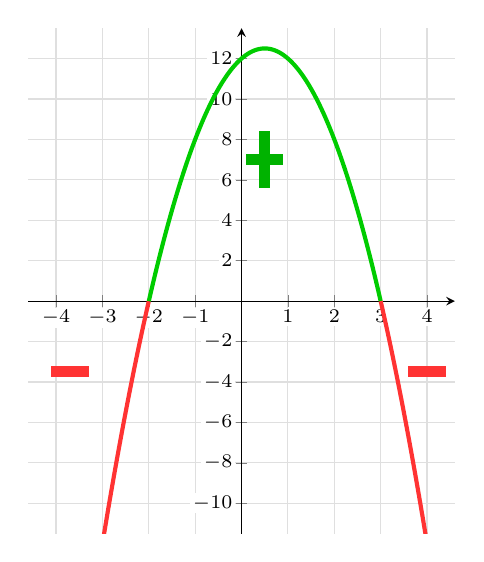
\begin{tikzpicture}
				\begin{axis}[repere, width=7cm, height=8cm,
					xmin=-4.6, xmax=4.6, ymin=-11.5, ymax=13.5,
					xtick={-4,...,4}, ytick={-10,-8,...,12}]
					\addplot[courbe, red!80!white, line width=1.5pt, domain=-3.2:-2] {-2*(x-3)*(x+2)};
					\addplot[courbe, green!80!black, line width=1.5pt, domain=-2:3] {-2*(x-3)*(x+2)};
					\addplot[courbe, red!80!white, line width=1.5pt, domain=3:4.2] {-2*(x-3)*(x+2)};
					\draw[green!70!black, line width=4pt] (axis cs:0.1,7) -- (axis cs:0.9,7);
					\draw[green!70!black, line width=4pt] (axis cs:0.5,5.6) -- (axis cs:0.5,8.4);
					\draw[red!80!white, line width=4pt] (axis cs:-4.1,-3.5) -- (axis cs:-3.3,-3.5);
					\draw[red!80!white, line width=4pt] (axis cs:3.6,-3.5) -- (axis cs:4.4,-3.5);
				\end{axis}
			\end{tikzpicture}
		\end{center}
		
	\end{bmethodet}
	
	

